\documentclass[12pt,a4paper]{article}
\usepackage[utf8]{vietnam}
\usepackage{amsmath,amssymb}
\usepackage[a4paper,left=2cm,right=1.8cm,top=1.8cm,bottom=1.8cm]{geometry}
\usepackage{tikz}
\usepackage{array,tabularx,longtable}
\usepackage{enumitem}
\setlength{\parindent}{0pt}
\setlength{\parskip}{3pt}
\linespread{1.15}
\pagestyle{plain}

% Phương án trắc nghiệm: 4 phương án trên 1 dòng / 2 dòng / mỗi phương án 1 dòng
\newcommand{\bonpa}[4]{\par\noindent\begin{tabularx}{\linewidth}{@{\hspace{0.6cm}}XXXX@{}}
\textbf{A.} #1 & \textbf{B.} #2 & \textbf{C.} #3 & \textbf{D.} #4\end{tabularx}\par}
\newcommand{\haipa}[4]{\par\noindent\begin{tabularx}{\linewidth}{@{\hspace{0.6cm}}XX@{}}
\textbf{A.} #1 & \textbf{B.} #2\\ \textbf{C.} #3 & \textbf{D.} #4\end{tabularx}\par}
\newcommand{\motpa}[4]{\par\hspace*{0.6cm}\textbf{A.} #1\par\hspace*{0.6cm}\textbf{B.} #2\par
\hspace*{0.6cm}\textbf{C.} #3\par\hspace*{0.6cm}\textbf{D.} #4\par}
\newcommand{\cau}[1]{\par\medskip\textbf{Câu #1.}~}
\newcommand{\bai}[2]{\par\medskip\textbf{Bài #1} \textit{(#2)}.~}
\newcommand{\y}[1]{\par\hspace*{0.6cm}#1}
\newcommand{\phan}[1]{\par\bigskip{\large\textbf{#1}}\par\smallskip}
\setlength{\extrarowheight}{2pt}

\begin{document}
\begin{center}
{\Large\textbf{BỘ 5 ĐỀ KIỂM TRA GIỮA HỌC KÌ I -- TOÁN 7}}\\[2pt]
Sách \textit{Kết nối tri thức với cuộc sống} -- Năm học 2026 -- 2027
\end{center}
\phan{1. Cấu trúc đề}
\begin{tabular}{|p{3.2cm}|p{6.2cm}|p{3.6cm}|c|}\hline
\textbf{Phần} & \textbf{Hình thức} & \textbf{Số câu / ý} & \textbf{Điểm}\\\hline
A. Trắc nghiệm (30\%) & Phần I. Nhiều phương án lựa chọn & 4 câu (câu 1 -- 4) & 1,0\\\cline{2-4}
 & Phần II. Đúng -- Sai & 1 câu, 4 ý (câu 5) & 1,0\\\cline{2-4}
 & Phần III. Trả lời ngắn & 4 câu (câu 6 -- 9) & 1,0\\\hline
B. Tự luận (70\%) & 6 bài & Bài 1 -- Bài 6 & 7,0\\\hline
\textbf{Tổng} & & \textbf{Thời gian: 90 phút} & \textbf{10,0}\\\hline
\end{tabular}

Mỗi câu (ý) trắc nghiệm đúng được 0,25 điểm.
\phan{2. Phạm vi kiến thức (theo PPCT Toán 7 -- KNTT)}
\textbf{Số và Đại số:} Chương I. Số hữu tỉ (Bài 1 -- Bài 4); Chương II -- Bài 5. Làm quen với số thập phân vô hạn tuần hoàn.

\textbf{Hình học:} Chương III. Góc và đường thẳng song song (Bài 8 -- Bài 11); Chương IV -- Bài 12. Tổng các góc trong một tam giác; Bài 13. Hai tam giác bằng nhau. Trường hợp bằng nhau thứ nhất (c.c.c).
\phan{3. Phân bố nội dung phần tự luận}
\begin{tabular}{|c|p{9cm}|p{3.4cm}|c|}\hline
\textbf{Bài} & \textbf{Nội dung} & \textbf{Mức độ} & \textbf{Điểm}\\\hline
1 & Thực hiện phép tính với số hữu tỉ, lũy thừa & Thông hiểu & 1,0\\\hline
2 & Tìm $x$ (quy tắc chuyển vế, lũy thừa) & Thông hiểu -- Vận dụng & 1,5\\\hline
3 & Bài toán thực tế với số hữu tỉ & Vận dụng & 1,0\\\hline
4 & Góc ở vị trí đặc biệt, tia phân giác, hai đường thẳng song song & Thông hiểu -- Vận dụng & 1,5\\\hline
5 & Tổng ba góc của tam giác; tam giác bằng nhau (c.c.c) & Thông hiểu -- Vận dụng & 1,5\\\hline
6 & Bài toán nâng cao & Vận dụng cao & 0,5\\\hline
\end{tabular}

\newpage
% ===================== ĐỀ SỐ 1 =====================
\noindent
\begin{minipage}[t]{0.38\linewidth}\centering
TRƯỜNG THCS \dotfill\\[2pt]
\textbf{ĐỀ SỐ 1}
\end{minipage}\hfill
\begin{minipage}[t]{0.6\linewidth}\centering
\textbf{ĐỀ KIỂM TRA GIỮA HỌC KÌ I}\\
\textbf{NĂM HỌC 2026 -- 2027}\\
\textbf{MÔN: TOÁN 7} -- Sách \textit{Kết nối tri thức với cuộc sống}\\
\textit{Thời gian làm bài: 90 phút (không kể thời gian giao đề)}
\end{minipage}

\medskip
Họ và tên: \dotfill\ Lớp: \makebox[2cm]{\dotfill}\ Số báo danh: \makebox[2.5cm]{\dotfill}
\phan{A. TRẮC NGHIỆM (3,0 điểm)}
\textbf{Phần I. Câu trắc nghiệm nhiều phương án lựa chọn} \textit{(1,0 điểm)}. Thí sinh trả lời từ câu 1 đến câu 4. Mỗi câu hỏi thí sinh chỉ chọn một phương án.
\cau{1} Số nào sau đây là số hữu tỉ âm?
\bonpa{$\dfrac{-3}{-5}$}{$0$}{$\dfrac{2}{-7}$}{$\dfrac{-4}{-9}$}
\cau{2} Kết quả của phép tính $\left(-\dfrac{2}{3}\right)^{3}$ là
\bonpa{$-\dfrac{8}{27}$}{$\dfrac{8}{27}$}{$-\dfrac{6}{9}$}{$-\dfrac{8}{9}$}
\cau{3} Phân số nào sau đây viết được dưới dạng số thập phân vô hạn tuần hoàn?
\bonpa{$\dfrac{3}{8}$}{$\dfrac{7}{20}$}{$\dfrac{5}{12}$}{$\dfrac{9}{25}$}
\cau{4} Cho hai đường thẳng $xx'$ và $yy'$ cắt nhau tại $O$. Biết $\widehat{xOy}=50^\circ$. Số đo của $\widehat{x'Oy'}$ là
\bonpa{$50^\circ$}{$130^\circ$}{$40^\circ$}{$180^\circ$}

\medskip\textbf{Phần II. Câu trắc nghiệm đúng sai} \textit{(1,0 điểm)}. Trong mỗi ý a), b), c), d) ở câu 5, thí sinh chọn đúng hoặc sai.
\cau{5} Cho hai số hữu tỉ $x=-\dfrac{3}{4}$ và $y=\dfrac{1}{2}$.
\y{a) $x\cdot y=\dfrac{3}{8}$.}
\y{b) $x<y$.}
\y{c) Số đối của $x$ là $\dfrac{4}{3}$.}
\y{d) $x+y=-\dfrac{1}{4}$.}

\medskip\textbf{Phần III. Câu trắc nghiệm trả lời ngắn} \textit{(1,0 điểm)}. Thí sinh trả lời từ câu 6 đến câu 9.
\cau{6} Tính giá trị của biểu thức $\dfrac{3^{5}}{3^{3}}-\left(\dfrac{1}{2}\right)^{0}$.
\cau{7} Tìm $x$, biết $x-\dfrac{1}{3}=\dfrac{2}{3}$.
\cau{8} Cho tam giác $ABC$ có $\widehat{A}=80^\circ$, $\widehat{B}=45^\circ$. Tính số đo $\widehat{C}$ (đơn vị: độ).
\cau{9} Cho tia $Oz$ là tia phân giác của $\widehat{xOy}$, biết $\widehat{xOy}=120^\circ$. Tính số đo $\widehat{xOz}$ (đơn vị: độ).
\phan{B. TỰ LUẬN (7,0 điểm)}
\bai{1}{1,0 điểm} Tính (hợp lí nếu có thể):
\par\noindent\begin{tabularx}{\linewidth}{@{\hspace{0.6cm}}XX@{}}a) $\dfrac{5}{9}\cdot\dfrac{-3}{7}+\dfrac{5}{9}\cdot\dfrac{-4}{7}$; & b) $\left(-\dfrac{1}{2}\right)^{2}+\dfrac{3}{4}:\dfrac{3}{2}-1{,}5$.\end{tabularx}
\bai{2}{1,5 điểm} Tìm $x$, biết:
\y{a) $x+\dfrac{2}{3}=-\dfrac{1}{6}$;}
\y{b) $\dfrac{3}{4}-2x=\dfrac{1}{4}$;}
\y{c) $\left(x-\dfrac{1}{2}\right)^{2}=\dfrac{9}{16}$.}
\bai{3}{1,0 điểm} Một cửa hàng có $150$ kg gạo. Ngày thứ nhất cửa hàng bán được $\dfrac{2}{5}$ số gạo. Ngày thứ hai cửa hàng bán được $\dfrac{3}{4}$ số gạo còn lại. Hỏi sau hai ngày, cửa hàng còn lại bao nhiêu ki-lô-gam gạo?
\bai{4}{1,5 điểm} Cho hình vẽ bên, đường thẳng $c$ cắt hai đường thẳng $a$ và $b$ lần lượt tại $A$ và $B$. Biết $\widehat{A_1}=115^\circ$, $\widehat{B_1}=65^\circ$.
\begin{center}
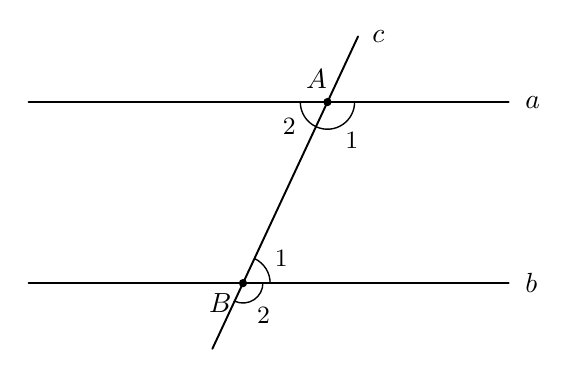
\begin{tikzpicture}[scale=1.15,line cap=round,line join=round]
  \draw[line width=0.7pt] (-0.300,2.000) -- (5.000,2.000);
  \draw[line width=0.7pt] (-0.300,0.000) -- (5.000,0.000);
  \draw[line width=0.7pt] (3.338,2.725) -- (1.729,-0.725);
  \node[anchor=west,inner sep=1pt] at (5.150,2.000) {$a$};
  \node[anchor=west,inner sep=1pt] at (5.150,0.000) {$b$};
  \node[anchor=west,inner sep=1pt] at (3.458,2.725) {$c$};
  \fill (3.000,2.000) circle (1.3pt);
  \node[anchor=center,inner sep=1pt] at (2.880,2.250) {$A$};
  \fill (2.067,0.000) circle (1.3pt);
  \node[anchor=center,inner sep=1pt] at (1.817,-0.220) {$B$};
  \draw[line width=0.5pt] (2.873,1.728) arc[start angle=-115,end angle=0,radius=0.300];
  \node[anchor=center,inner sep=1pt] at (3.269,1.578) {{\small 1}};
  \draw[line width=0.5pt] (2.700,2.000) arc[start angle=-180,end angle=-115,radius=0.300];
  \node[anchor=center,inner sep=1pt] at (2.578,1.731) {{\small 2}};
  \draw[line width=0.5pt] (2.367,0.000) arc[start angle=0,end angle=65,radius=0.300];
  \node[anchor=center,inner sep=1pt] at (2.489,0.269) {{\small 1}};
  \draw[line width=0.5pt] (1.974,-0.199) arc[start angle=-115,end angle=0,radius=0.220];
  \node[anchor=center,inner sep=1pt] at (2.293,-0.354) {{\small 2}};
\end{tikzpicture}
\end{center}
\y{a) Chứng minh $a\parallel b$.}
\y{b) Tính số đo $\widehat{B_2}$.}
\y{c) Đường thẳng $d$ vuông góc với đường thẳng $a$. Chứng minh $d\perp b$.}
\bai{5}{1,5 điểm} Cho tam giác $ABC$ có $AB=AC$. Gọi $M$ là trung điểm của đoạn thẳng $BC$.
\y{a) Chứng minh $\triangle ABM=\triangle ACM$.}
\y{b) Chứng minh $AM$ là tia phân giác của $\widehat{BAC}$.}
\y{c) Chứng minh $AM\perp BC$.}
\bai{6}{0,5 điểm} Tính tổng $A=\dfrac{1}{1\cdot 2}+\dfrac{1}{2\cdot 3}+\dfrac{1}{3\cdot 4}+\ldots+\dfrac{1}{99\cdot 100}$.

\bigskip\begin{center}\textbf{--------- HẾT ---------}\\
\textit{Giáo viên coi kiểm tra không giải thích gì thêm.}\end{center}

\newpage
\begin{center}{\large\textbf{HƯỚNG DẪN CHẤM -- ĐỀ SỐ 1}}\end{center}
\phan{A. TRẮC NGHIỆM (3,0 điểm)}
\textbf{Phần I.} Mỗi câu trả lời đúng được 0,25 điểm.

\begin{tabular}{|l|*{4}{>{\centering\arraybackslash}p{2cm}|}}\hline
Câu & 1 & 2 & 3 & 4 \\ \hline
Đáp án & \textbf{C} & \textbf{A} & \textbf{C} & \textbf{A} \\ \hline
\end{tabular}

\textbf{Phần II.} Mỗi ý trả lời đúng được 0,25 điểm.

\begin{tabular}{|l|*{4}{>{\centering\arraybackslash}p{2cm}|}}\hline
Câu 5 & a) & b) & c) & d) \\ \hline
Đáp án & \textbf{Sai} & \textbf{Đúng} & \textbf{Sai} & \textbf{Đúng} \\ \hline
\end{tabular}

\textbf{Phần III.} Mỗi câu trả lời đúng được 0,25 điểm.

\begin{tabular}{|l|*{4}{>{\centering\arraybackslash}p{2cm}|}}\hline
Câu & 6 & 7 & 8 & 9 \\ \hline
Đáp án & \textbf{8} & \textbf{1} & \textbf{55} & \textbf{60} \\ \hline
\end{tabular}

\phan{B. TỰ LUẬN (7,0 điểm)}
\begin{longtable}{|>{\bfseries}c|p{0.76\linewidth}|>{\centering\arraybackslash}p{1.3cm}|}\hline
Bài & \multicolumn{1}{c|}{\textbf{Nội dung}} & \textbf{Điểm} \\ \hline\endhead
1a & \rule{0pt}{4ex}$\dfrac{5}{9}\cdot\dfrac{-3}{7}+\dfrac{5}{9}\cdot\dfrac{-4}{7}=\dfrac{5}{9}\cdot\left(\dfrac{-3}{7}+\dfrac{-4}{7}\right)$\rule[-2.4ex]{0pt}{0pt} & 0,25 \\ \hline
 & \rule{0pt}{4ex}$=\dfrac{5}{9}\cdot(-1)=-\dfrac{5}{9}$\rule[-2.4ex]{0pt}{0pt} & 0,25 \\ \hline
1b & \rule{0pt}{4ex}$\left(-\dfrac{1}{2}\right)^{2}+\dfrac{3}{4}:\dfrac{3}{2}-1{,}5=\dfrac{1}{4}+\dfrac{3}{4}\cdot\dfrac{2}{3}-\dfrac{3}{2}=\dfrac{1}{4}+\dfrac{1}{2}-\dfrac{3}{2}$\rule[-2.4ex]{0pt}{0pt} & 0,25 \\ \hline
 & \rule{0pt}{4ex}$=\dfrac{1}{4}-1=-\dfrac{3}{4}$\rule[-2.4ex]{0pt}{0pt} & 0,25 \\ \hline
2a & \rule{0pt}{4ex}$x=-\dfrac{1}{6}-\dfrac{2}{3}=-\dfrac{1}{6}-\dfrac{4}{6}$\rule[-2.4ex]{0pt}{0pt} & 0,25 \\ \hline
 & \rule{0pt}{4ex}$x=-\dfrac{5}{6}$. Vậy $x=-\dfrac{5}{6}$.\rule[-2.4ex]{0pt}{0pt} & 0,25 \\ \hline
2b & \rule{0pt}{4ex}$2x=\dfrac{3}{4}-\dfrac{1}{4}=\dfrac{1}{2}$\rule[-2.4ex]{0pt}{0pt} & 0,25 \\ \hline
 & \rule{0pt}{4ex}$x=\dfrac{1}{2}:2=\dfrac{1}{4}$. Vậy $x=\dfrac{1}{4}$.\rule[-2.4ex]{0pt}{0pt} & 0,25 \\ \hline
2c & \rule{0pt}{4ex}$\left(x-\dfrac{1}{2}\right)^{2}=\left(\dfrac{3}{4}\right)^{2}=\left(-\dfrac{3}{4}\right)^{2}$ nên $x-\dfrac{1}{2}=\dfrac{3}{4}$ hoặc $x-\dfrac{1}{2}=-\dfrac{3}{4}$\rule[-2.4ex]{0pt}{0pt} & 0,25 \\ \hline
 & \rule{0pt}{4ex}$x=\dfrac{5}{4}$ hoặc $x=-\dfrac{1}{4}$. Vậy $x\in\left\{\dfrac{5}{4};-\dfrac{1}{4}\right\}$.\rule[-2.4ex]{0pt}{0pt} & 0,25 \\ \hline
3 & \rule{0pt}{4ex}Số gạo bán ngày thứ nhất: $150\cdot\dfrac{2}{5}=60$ (kg).\rule[-2.4ex]{0pt}{0pt} & 0,25 \\ \hline
 & Số gạo còn lại sau ngày thứ nhất: $150-60=90$ (kg). & 0,25 \\ \hline
 & \rule{0pt}{4ex}Số gạo bán ngày thứ hai: $90\cdot\dfrac{3}{4}=67{,}5$ (kg).\rule[-2.4ex]{0pt}{0pt} & 0,25 \\ \hline
 & Số gạo còn lại sau hai ngày: $90-67{,}5=22{,}5$ (kg). & 0,25 \\ \hline
4a & Ta có $\widehat{A_1}+\widehat{A_2}=180^\circ$ (hai góc kề bù) nên $\widehat{A_2}=180^\circ-115^\circ=65^\circ$. & 0,25 \\ \hline
 & Do đó $\widehat{A_2}=\widehat{B_1}=65^\circ$, mà $\widehat{A_2}$ và $\widehat{B_1}$ ở vị trí so le trong nên $a\parallel b$. & 0,25 \\ \hline
4b & $\widehat{B_1}$ và $\widehat{B_2}$ là hai góc kề bù nên $\widehat{B_1}+\widehat{B_2}=180^\circ$ & 0,25 \\ \hline
 & $\widehat{B_2}=180^\circ-65^\circ=115^\circ$. & 0,25 \\ \hline
4c & Ta có $d\perp a$ và $a\parallel b$ & 0,25 \\ \hline
 & nên $d\perp b$ (một đường thẳng vuông góc với một trong hai đường thẳng song song thì vuông góc với đường thẳng kia). & 0,25 \\ \hline
5 & Vẽ hình, ghi GT – KL đúng. \newline \textit{(Hình vẽ ở cuối hướng dẫn chấm)} & 0,25 \\ \hline
5a & Xét $\triangle ABM$ và $\triangle ACM$ có: $AB=AC$ (gt); $BM=CM$ ($M$ là trung điểm $BC$); $AM$ là cạnh chung. & 0,25 \\ \hline
 & Do đó $\triangle ABM=\triangle ACM$ (c.c.c). & 0,25 \\ \hline
5b & Vì $\triangle ABM=\triangle ACM$ nên $\widehat{BAM}=\widehat{CAM}$ (hai góc tương ứng). Mà tia $AM$ nằm giữa hai tia $AB$, $AC$ nên $AM$ là tia phân giác của $\widehat{BAC}$. & 0,25 \\ \hline
5c & Vì $\triangle ABM=\triangle ACM$ nên $\widehat{AMB}=\widehat{AMC}$ (hai góc tương ứng). Mà $\widehat{AMB}+\widehat{AMC}=180^\circ$ (hai góc kề bù) & 0,25 \\ \hline
 & nên $\widehat{AMB}=\widehat{AMC}=90^\circ$. Vậy $AM\perp BC$. & 0,25 \\ \hline
6 & \rule{0pt}{4ex}$A=\left(1-\dfrac{1}{2}\right)+\left(\dfrac{1}{2}-\dfrac{1}{3}\right)+\ldots+\left(\dfrac{1}{99}-\dfrac{1}{100}\right)$ (vì $\dfrac{1}{n(n+1)}=\dfrac{1}{n}-\dfrac{1}{n+1}$)\rule[-2.4ex]{0pt}{0pt} & 0,25 \\ \hline
 & \rule{0pt}{4ex}$A=1-\dfrac{1}{100}=\dfrac{99}{100}$.\rule[-2.4ex]{0pt}{0pt} & 0,25 \\ \hline
\end{longtable}
\textit{Lưu ý: Học sinh làm cách khác đúng vẫn cho điểm tối đa theo thang điểm tương ứng. Bài hình không vẽ hình hoặc vẽ hình sai không chấm phần tương ứng.}

\textbf{Hình vẽ bài 5:}
\begin{center}
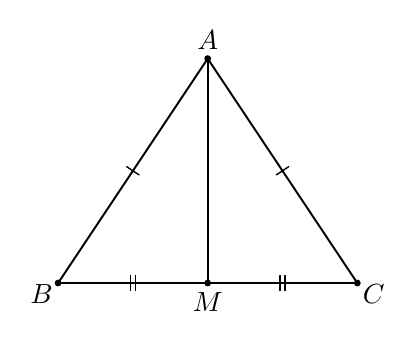
\begin{tikzpicture}[scale=0.95,line cap=round,line join=round]
  \draw[line width=0.7pt] (2.000,3.000) -- (0.000,0.000);
  \draw[line width=0.7pt] (2.000,3.000) -- (4.000,0.000);
  \draw[line width=0.7pt] (0.000,0.000) -- (4.000,0.000);
  \draw[line width=0.7pt] (2.000,3.000) -- (2.000,0.000);
  \draw[line width=0.5pt] (0.917,1.555) -- (1.083,1.445);
  \draw[line width=0.5pt] (2.917,1.445) -- (3.083,1.555);
  \draw[line width=0.5pt] (0.965,-0.100) -- (0.965,0.100);
  \draw[line width=0.5pt] (1.035,-0.100) -- (1.035,0.100);
  \draw[line width=0.5pt] (2.965,-0.100) -- (2.965,0.100);
  \draw[line width=0.5pt] (3.035,-0.100) -- (3.035,0.100);
  \fill (2.000,3.000) circle (1.3pt);
  \node[anchor=center,inner sep=1pt] at (2.000,3.250) {$A$};
  \fill (0.000,0.000) circle (1.3pt);
  \node[anchor=center,inner sep=1pt] at (-0.220,-0.150) {$B$};
  \fill (4.000,0.000) circle (1.3pt);
  \node[anchor=center,inner sep=1pt] at (4.220,-0.150) {$C$};
  \fill (2.000,0.000) circle (1.3pt);
  \node[anchor=center,inner sep=1pt] at (2.000,-0.250) {$M$};
\end{tikzpicture}
\end{center}

\newpage
% ===================== ĐỀ SỐ 2 =====================
\noindent
\begin{minipage}[t]{0.38\linewidth}\centering
TRƯỜNG THCS \dotfill\\[2pt]
\textbf{ĐỀ SỐ 2}
\end{minipage}\hfill
\begin{minipage}[t]{0.6\linewidth}\centering
\textbf{ĐỀ KIỂM TRA GIỮA HỌC KÌ I}\\
\textbf{NĂM HỌC 2026 -- 2027}\\
\textbf{MÔN: TOÁN 7} -- Sách \textit{Kết nối tri thức với cuộc sống}\\
\textit{Thời gian làm bài: 90 phút (không kể thời gian giao đề)}
\end{minipage}

\medskip
Họ và tên: \dotfill\ Lớp: \makebox[2cm]{\dotfill}\ Số báo danh: \makebox[2.5cm]{\dotfill}
\phan{A. TRẮC NGHIỆM (3,0 điểm)}
\textbf{Phần I. Câu trắc nghiệm nhiều phương án lựa chọn} \textit{(1,0 điểm)}. Thí sinh trả lời từ câu 1 đến câu 4. Mỗi câu hỏi thí sinh chỉ chọn một phương án.
\cau{1} Số đối của số hữu tỉ $-\dfrac{5}{7}$ là
\bonpa{$\dfrac{5}{7}$}{$-\dfrac{5}{7}$}{$\dfrac{7}{5}$}{$-\dfrac{7}{5}$}
\cau{2} Với $x$ là số hữu tỉ khác $0$, kết quả của phép tính $x^{5}\cdot x^{3}$ là
\bonpa{$x^{15}$}{$x^{8}$}{$x^{2}$}{$2x^{8}$}
\cau{3} Phân số $\dfrac{1}{3}$ được viết dưới dạng số thập phân là
\bonpa{$0{,}3$}{$0{,}(3)$}{$0{,}33$}{$3{,}(3)$}
\cau{4} Nếu một đường thẳng cắt hai đường thẳng song song thì hai góc so le trong
\bonpa{bằng nhau.}{bù nhau.}{phụ nhau.}{kề bù.}

\medskip\textbf{Phần II. Câu trắc nghiệm đúng sai} \textit{(1,0 điểm)}. Trong mỗi ý a), b), c), d) ở câu 5, thí sinh chọn đúng hoặc sai.
\cau{5} Cho $\widehat{xOy}=80^\circ$, tia $Ot$ là tia phân giác của $\widehat{xOy}$. Vẽ tia $Ox'$ là tia đối của tia $Ox$.
\y{a) $\widehat{xOt}=40^\circ$.}
\y{b) $\widehat{x'Oy}=100^\circ$.}
\y{c) $\widehat{x'Ot}=150^\circ$.}
\y{d) $\widehat{xOy}$ và $\widehat{x'Oy}$ là hai góc đối đỉnh.}

\medskip\textbf{Phần III. Câu trắc nghiệm trả lời ngắn} \textit{(1,0 điểm)}. Thí sinh trả lời từ câu 6 đến câu 9.
\cau{6} Tính giá trị của biểu thức $\left(-\dfrac{1}{3}\right)^{2}\cdot 27$.
\cau{7} Tìm $x$, biết $\dfrac{x}{4}=-\dfrac{3}{2}$.
\cau{8} Cho tam giác $ABC$ vuông tại $A$ có $\widehat{B}=35^\circ$. Tính số đo $\widehat{C}$ (đơn vị: độ).
\cau{9} Cho $\triangle ABC=\triangle DEF$, biết $AB=5$ cm, $BC=7$ cm, $DF=6$ cm. Tính chu vi tam giác $DEF$ (đơn vị: cm).
\phan{B. TỰ LUẬN (7,0 điểm)}
\bai{1}{1,0 điểm} Tính (hợp lí nếu có thể):
\par\noindent\begin{tabularx}{\linewidth}{@{\hspace{0.6cm}}XX@{}}a) $\dfrac{-7}{13}\cdot\dfrac{5}{11}+\dfrac{-7}{13}\cdot\dfrac{6}{11}+1\dfrac{7}{13}$; & b) $\left(\dfrac{2}{3}\right)^{3}\cdot\left(\dfrac{3}{2}\right)^{2}-\dfrac{1}{3}$.\end{tabularx}
\bai{2}{1,5 điểm} Tìm $x$, biết:
\y{a) $\dfrac{2}{5}x=-\dfrac{4}{15}$;}
\y{b) $\dfrac{1}{2}-\left(x+\dfrac{1}{3}\right)=\dfrac{3}{4}$;}
\y{c) $2^{x}+2^{x+2}=40$.}
\bai{3}{1,0 điểm} Lớp 7A có $40$ học sinh. Số học sinh xếp loại Tốt chiếm $\dfrac{1}{4}$ số học sinh cả lớp. Số học sinh xếp loại Khá bằng $\dfrac{3}{5}$ số học sinh còn lại, các học sinh còn lại xếp loại Đạt. Tính số học sinh mỗi loại của lớp 7A.
\bai{4}{1,5 điểm} Cho hình vẽ bên, biết $Ax\parallel By$, $\widehat{xAO}=40^\circ$, $\widehat{OBy}=30^\circ$. Vẽ tia $Ot$ nằm trong $\widehat{AOB}$ sao cho $Ot\parallel Ax$.
\begin{center}
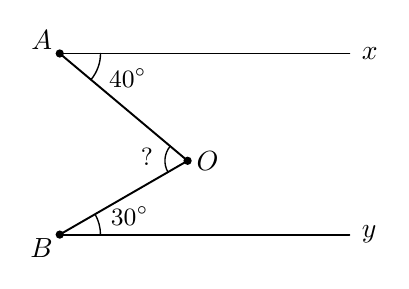
\begin{tikzpicture}[scale=1.15,line cap=round,line join=round]
  \draw[line width=0.7pt] (0.000,2.000) -- (3.200,2.000);
  \draw[line width=0.7pt] (0.000,0.000) -- (3.200,0.000);
  \draw[line width=0.7pt] (0.000,2.000) -- (1.412,0.815);
  \draw[line width=0.7pt] (0.000,0.000) -- (1.412,0.815);
  \node[anchor=west,inner sep=1pt] at (3.300,2.000) {$x$};
  \node[anchor=west,inner sep=1pt] at (3.300,0.000) {$y$};
  \fill (0.000,2.000) circle (1.3pt);
  \node[anchor=center,inner sep=1pt] at (-0.200,2.150) {$A$};
  \fill (0.000,0.000) circle (1.3pt);
  \node[anchor=center,inner sep=1pt] at (-0.200,-0.150) {$B$};
  \fill (1.412,0.815) circle (1.3pt);
  \node[anchor=center,inner sep=1pt] at (1.632,0.815) {$O$};
  \draw[line width=0.5pt] (0.345,1.711) arc[start angle=-40,end angle=0,radius=0.450];
  \node[anchor=center,inner sep=1pt] at (0.752,1.726) {{\small $40^\circ$}};
  \draw[line width=0.5pt] (0.450,0.000) arc[start angle=0,end angle=30,radius=0.450];
  \node[anchor=center,inner sep=1pt] at (0.773,0.207) {{\small $30^\circ$}};
  \draw[line width=0.5pt] (1.220,0.976) arc[start angle=140,end angle=210,radius=0.250];
  \node[anchor=center,inner sep=1pt] at (0.964,0.854) {{\small ?}};
\end{tikzpicture}
\end{center}
\y{a) Chứng minh $Ot\parallel By$.}
\y{b) Tính số đo $\widehat{AOB}$.}
\y{c) Vẽ tia $Om$ là tia phân giác của $\widehat{AOB}$. Tính số đo $\widehat{mOt}$.}
\bai{5}{1,5 điểm} Cho $\widehat{xOy}$ nhọn. Trên tia $Ox$ lấy điểm $A$, trên tia $Oy$ lấy điểm $B$ sao cho $OA=OB$. Lấy điểm $C$ nằm trong $\widehat{xOy}$ sao cho $CA=CB$.
\y{a) Chứng minh $\triangle OAC=\triangle OBC$.}
\y{b) Chứng minh $OC$ là tia phân giác của $\widehat{xOy}$.}
\y{c) Biết $\widehat{xOy}=60^\circ$ và $\widehat{OAC}=100^\circ$. Tính số đo $\widehat{OCB}$.}
\bai{6}{0,5 điểm} So sánh $2^{300}$ và $3^{200}$.

\bigskip\begin{center}\textbf{--------- HẾT ---------}\\
\textit{Giáo viên coi kiểm tra không giải thích gì thêm.}\end{center}

\newpage
\begin{center}{\large\textbf{HƯỚNG DẪN CHẤM -- ĐỀ SỐ 2}}\end{center}
\phan{A. TRẮC NGHIỆM (3,0 điểm)}
\textbf{Phần I.} Mỗi câu trả lời đúng được 0,25 điểm.

\begin{tabular}{|l|*{4}{>{\centering\arraybackslash}p{2cm}|}}\hline
Câu & 1 & 2 & 3 & 4 \\ \hline
Đáp án & \textbf{A} & \textbf{B} & \textbf{B} & \textbf{A} \\ \hline
\end{tabular}

\textbf{Phần II.} Mỗi ý trả lời đúng được 0,25 điểm.

\begin{tabular}{|l|*{4}{>{\centering\arraybackslash}p{2cm}|}}\hline
Câu 5 & a) & b) & c) & d) \\ \hline
Đáp án & \textbf{Đúng} & \textbf{Đúng} & \textbf{Sai} & \textbf{Sai} \\ \hline
\end{tabular}

\textbf{Phần III.} Mỗi câu trả lời đúng được 0,25 điểm.

\begin{tabular}{|l|*{4}{>{\centering\arraybackslash}p{2cm}|}}\hline
Câu & 6 & 7 & 8 & 9 \\ \hline
Đáp án & \textbf{3} & \textbf{$-$6} & \textbf{55} & \textbf{18} \\ \hline
\end{tabular}

\phan{B. TỰ LUẬN (7,0 điểm)}
\begin{longtable}{|>{\bfseries}c|p{0.76\linewidth}|>{\centering\arraybackslash}p{1.3cm}|}\hline
Bài & \multicolumn{1}{c|}{\textbf{Nội dung}} & \textbf{Điểm} \\ \hline\endhead
1a & \rule{0pt}{4ex}$\dfrac{-7}{13}\cdot\left(\dfrac{5}{11}+\dfrac{6}{11}\right)+1\dfrac{7}{13}=\dfrac{-7}{13}\cdot 1+\dfrac{20}{13}$\rule[-2.4ex]{0pt}{0pt} & 0,25 \\ \hline
 & \rule{0pt}{4ex}$=\dfrac{13}{13}=1$\rule[-2.4ex]{0pt}{0pt} & 0,25 \\ \hline
1b & \rule{0pt}{4ex}$\dfrac{8}{27}\cdot\dfrac{9}{4}-\dfrac{1}{3}=\dfrac{2}{3}-\dfrac{1}{3}$\rule[-2.4ex]{0pt}{0pt} & 0,25 \\ \hline
 & \rule{0pt}{4ex}$=\dfrac{1}{3}$\rule[-2.4ex]{0pt}{0pt} & 0,25 \\ \hline
2a & \rule{0pt}{4ex}$x=-\dfrac{4}{15}:\dfrac{2}{5}=-\dfrac{4}{15}\cdot\dfrac{5}{2}$\rule[-2.4ex]{0pt}{0pt} & 0,25 \\ \hline
 & \rule{0pt}{4ex}$x=-\dfrac{2}{3}$. Vậy $x=-\dfrac{2}{3}$.\rule[-2.4ex]{0pt}{0pt} & 0,25 \\ \hline
2b & \rule{0pt}{4ex}$x+\dfrac{1}{3}=\dfrac{1}{2}-\dfrac{3}{4}=-\dfrac{1}{4}$\rule[-2.4ex]{0pt}{0pt} & 0,25 \\ \hline
 & \rule{0pt}{4ex}$x=-\dfrac{1}{4}-\dfrac{1}{3}=-\dfrac{7}{12}$. Vậy $x=-\dfrac{7}{12}$.\rule[-2.4ex]{0pt}{0pt} & 0,25 \\ \hline
2c & $2^{x}+2^{x}\cdot 2^{2}=40$ hay $2^{x}\cdot(1+4)=40$, suy ra $2^{x}=8$ & 0,25 \\ \hline
 & $2^{x}=2^{3}$ nên $x=3$. Vậy $x=3$. & 0,25 \\ \hline
3 & \rule{0pt}{4ex}Số học sinh xếp loại Tốt: $40\cdot\dfrac{1}{4}=10$ (học sinh).\rule[-2.4ex]{0pt}{0pt} & 0,25 \\ \hline
 & Số học sinh còn lại: $40-10=30$ (học sinh). & 0,25 \\ \hline
 & \rule{0pt}{4ex}Số học sinh xếp loại Khá: $30\cdot\dfrac{3}{5}=18$ (học sinh).\rule[-2.4ex]{0pt}{0pt} & 0,25 \\ \hline
 & Số học sinh xếp loại Đạt: $30-18=12$ (học sinh). & 0,25 \\ \hline
4a & Ta có $Ot\parallel Ax$ và $Ax\parallel By$ & 0,25 \\ \hline
 & nên $Ot\parallel By$ (hai đường thẳng phân biệt cùng song song với đường thẳng thứ ba). & 0,25 \\ \hline
4b & Vì $Ot\parallel Ax$ nên $\widehat{AOt}=\widehat{xAO}=40^\circ$ (so le trong); vì $Ot\parallel By$ nên $\widehat{tOB}=\widehat{OBy}=30^\circ$ (so le trong). & 0,25 \\ \hline
 & Tia $Ot$ nằm giữa hai tia $OA$, $OB$ nên $\widehat{AOB}=\widehat{AOt}+\widehat{tOB}=40^\circ+30^\circ=70^\circ$. & 0,25 \\ \hline
4c & \rule{0pt}{4ex}$Om$ là tia phân giác của $\widehat{AOB}$ nên $\widehat{AOm}=\dfrac{70^\circ}{2}=35^\circ$.\rule[-2.4ex]{0pt}{0pt} & 0,25 \\ \hline
 & Vì $\widehat{AOm}<\widehat{AOt}$ nên tia $Om$ nằm giữa hai tia $OA$, $Ot$; suy ra $\widehat{mOt}=40^\circ-35^\circ=5^\circ$. & 0,25 \\ \hline
5 & Vẽ hình, ghi GT – KL đúng. \newline \textit{(Hình vẽ ở cuối hướng dẫn chấm)} & 0,25 \\ \hline
5a & Xét $\triangle OAC$ và $\triangle OBC$ có: $OA=OB$ (gt); $CA=CB$ (gt); $OC$ là cạnh chung. & 0,25 \\ \hline
 & Do đó $\triangle OAC=\triangle OBC$ (c.c.c). & 0,25 \\ \hline
5b & Từ câu a suy ra $\widehat{AOC}=\widehat{BOC}$ (hai góc tương ứng). Mà tia $OC$ nằm giữa hai tia $Ox$, $Oy$ nên $OC$ là tia phân giác của $\widehat{xOy}$. & 0,25 \\ \hline
5c & \rule{0pt}{4ex}$\widehat{AOC}=\dfrac{60^\circ}{2}=30^\circ$. Trong $\triangle OAC$: $\widehat{OCA}=180^\circ-100^\circ-30^\circ=50^\circ$.\rule[-2.4ex]{0pt}{0pt} & 0,25 \\ \hline
 & Vì $\triangle OAC=\triangle OBC$ nên $\widehat{OCB}=\widehat{OCA}=50^\circ$. & 0,25 \\ \hline
6 & $2^{300}=\left(2^{3}\right)^{100}=8^{100}$; $3^{200}=\left(3^{2}\right)^{100}=9^{100}$. & 0,25 \\ \hline
 & Vì $8^{100}<9^{100}$ nên $2^{300}<3^{200}$. & 0,25 \\ \hline
\end{longtable}
\textit{Lưu ý: Học sinh làm cách khác đúng vẫn cho điểm tối đa theo thang điểm tương ứng. Bài hình không vẽ hình hoặc vẽ hình sai không chấm phần tương ứng.}

\textbf{Hình vẽ bài 5:}
\begin{center}
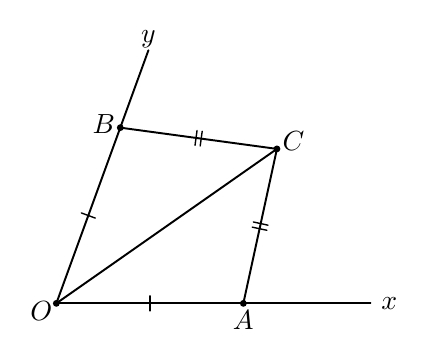
\begin{tikzpicture}[scale=0.95,line cap=round,line join=round]
  \draw[line width=0.7pt] (0.000,0.000) -- (4.200,0.000);
  \draw[line width=0.7pt] (0.000,0.000) -- (1.231,3.383);
  \draw[line width=0.7pt] (0.000,0.000) -- (2.949,2.065);
  \draw[line width=0.7pt] (2.500,0.000) -- (2.949,2.065);
  \draw[line width=0.7pt] (0.855,2.349) -- (2.949,2.065);
  \draw[line width=0.5pt] (1.250,-0.100) -- (1.250,0.100);
  \draw[line width=0.5pt] (0.521,1.140) -- (0.334,1.209);
  \draw[line width=0.5pt] (2.815,0.977) -- (2.619,1.019);
  \draw[line width=0.5pt] (2.830,1.045) -- (2.634,1.088);
  \draw[line width=0.5pt] (1.854,2.113) -- (1.881,2.311);
  \draw[line width=0.5pt] (1.923,2.103) -- (1.950,2.301);
  \node[anchor=west,inner sep=1pt] at (4.300,0.000) {$x$};
  \node[anchor=center,inner sep=1pt] at (1.231,3.533) {$y$};
  \fill (0.000,0.000) circle (1.3pt);
  \node[anchor=center,inner sep=1pt] at (-0.200,-0.100) {$O$};
  \fill (2.500,0.000) circle (1.3pt);
  \node[anchor=center,inner sep=1pt] at (2.500,-0.220) {$A$};
  \fill (0.855,2.349) circle (1.3pt);
  \node[anchor=center,inner sep=1pt] at (0.635,2.399) {$B$};
  \fill (2.949,2.065) circle (1.3pt);
  \node[anchor=center,inner sep=1pt] at (3.169,2.165) {$C$};
\end{tikzpicture}
\end{center}

\newpage
% ===================== ĐỀ SỐ 3 =====================
\noindent
\begin{minipage}[t]{0.38\linewidth}\centering
TRƯỜNG THCS \dotfill\\[2pt]
\textbf{ĐỀ SỐ 3}
\end{minipage}\hfill
\begin{minipage}[t]{0.6\linewidth}\centering
\textbf{ĐỀ KIỂM TRA GIỮA HỌC KÌ I}\\
\textbf{NĂM HỌC 2026 -- 2027}\\
\textbf{MÔN: TOÁN 7} -- Sách \textit{Kết nối tri thức với cuộc sống}\\
\textit{Thời gian làm bài: 90 phút (không kể thời gian giao đề)}
\end{minipage}

\medskip
Họ và tên: \dotfill\ Lớp: \makebox[2cm]{\dotfill}\ Số báo danh: \makebox[2.5cm]{\dotfill}
\phan{A. TRẮC NGHIỆM (3,0 điểm)}
\textbf{Phần I. Câu trắc nghiệm nhiều phương án lựa chọn} \textit{(1,0 điểm)}. Thí sinh trả lời từ câu 1 đến câu 4. Mỗi câu hỏi thí sinh chỉ chọn một phương án.
\cau{1} Phân số nào sau đây biểu diễn số hữu tỉ $-0{,}75$?
\bonpa{$\dfrac{3}{4}$}{$\dfrac{-3}{4}$}{$\dfrac{-7}{5}$}{$\dfrac{-4}{3}$}
\cau{2} Kết quả của phép tính $\left(\dfrac{1}{2}\right)^{6}:\left(\dfrac{1}{2}\right)^{2}$ là
\bonpa{$\left(\dfrac{1}{2}\right)^{3}$}{$\left(\dfrac{1}{2}\right)^{4}$}{$\left(\dfrac{1}{2}\right)^{8}$}{$\left(\dfrac{1}{2}\right)^{12}$}
\cau{3} Làm tròn số $3{,}14159$ đến hàng phần trăm ta được
\bonpa{$3{,}14$}{$3{,}15$}{$3{,}1$}{$3{,}142$}
\cau{4} Trong một tam giác vuông, hai góc nhọn
\bonpa{bằng nhau.}{bù nhau.}{phụ nhau.}{kề bù.}

\medskip\textbf{Phần II. Câu trắc nghiệm đúng sai} \textit{(1,0 điểm)}. Trong mỗi ý a), b), c), d) ở câu 5, thí sinh chọn đúng hoặc sai.
\cau{5} Xét tính đúng, sai của các khẳng định sau:
\y{a) $\left(-\dfrac{1}{2}\right)^{4}=\dfrac{1}{16}$.}
\y{b) $3^{2}\cdot 3^{3}=3^{6}$.}
\y{c) $\left(2^{3}\right)^{2}=2^{6}$.}
\y{d) $\left(-\dfrac{2}{3}\right)^{0}=0$.}

\medskip\textbf{Phần III. Câu trắc nghiệm trả lời ngắn} \textit{(1,0 điểm)}. Thí sinh trả lời từ câu 6 đến câu 9.
\cau{6} Tính $\dfrac{-5}{6}+\dfrac{1}{3}$ (viết kết quả dưới dạng số thập phân).
\cau{7} Tìm $x$, biết $x:\dfrac{2}{3}=-\dfrac{9}{4}$ (viết kết quả dưới dạng số thập phân).
\cau{8} Đường thẳng $c$ cắt hai đường thẳng song song $a$ và $b$. Biết một góc tạo bởi $c$ và $a$ bằng $72^\circ$. Tính số đo góc đồng vị với góc đó (đơn vị: độ).
\cau{9} Cho $\triangle MNP=\triangle HIK$, biết $\widehat{M}=50^\circ$, $\widehat{I}=70^\circ$. Tính số đo $\widehat{P}$ (đơn vị: độ).
\phan{B. TỰ LUẬN (7,0 điểm)}
\bai{1}{1,0 điểm} Tính (hợp lí nếu có thể):
\y{a) $\dfrac{15}{34}+\dfrac{7}{21}+\dfrac{19}{34}-1\dfrac{15}{17}+\dfrac{2}{3}$;}
\y{b) $(-2)^{3}\cdot\left(\dfrac{1}{2}\right)^{2}+\left(\dfrac{3}{4}-\dfrac{1}{4}\right):\dfrac{1}{8}$.}
\bai{2}{1,5 điểm} Tìm $x$, biết:
\y{a) $x-\dfrac{3}{5}=\dfrac{1}{2}$;}
\y{b) $\dfrac{2}{3}x+\dfrac{1}{4}=\dfrac{5}{12}$;}
\y{c) $(2x-1)^{3}=-8$.}
\bai{3}{1,0 điểm} Một mảnh vườn hình chữ nhật có chiều dài $12{,}5$ m, chiều rộng bằng $\dfrac{4}{5}$ chiều dài.
\y{a) Tính chu vi và diện tích mảnh vườn.}
\y{b) Người ta dùng $\dfrac{3}{5}$ diện tích mảnh vườn để trồng rau. Tính diện tích phần đất trồng rau.}
\bai{4}{1,5 điểm} Cho hình vẽ bên, biết $a\perp c$, $b\perp c$, đường thẳng $d$ cắt $a$, $b$ lần lượt tại $M$, $N$ và $\widehat{M_1}=120^\circ$.
\begin{center}
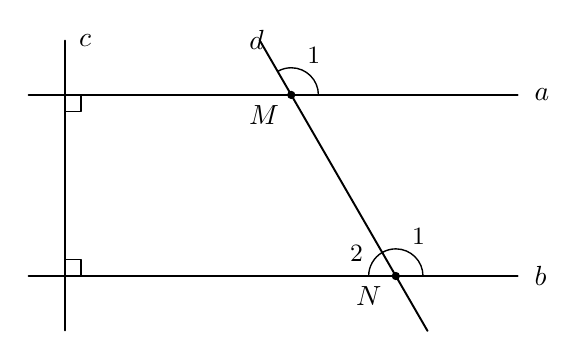
\begin{tikzpicture}[scale=1.15,line cap=round,line join=round]
  \draw[line width=0.7pt] (0.000,-0.600) -- (0.000,2.600);
  \draw[line width=0.7pt] (-0.400,2.000) -- (5.000,2.000);
  \draw[line width=0.7pt] (-0.400,0.000) -- (5.000,0.000);
  \node[anchor=west,inner sep=1pt] at (0.120,2.600) {$c$};
  \node[anchor=west,inner sep=1pt] at (5.150,2.000) {$a$};
  \node[anchor=west,inner sep=1pt] at (5.150,0.000) {$b$};
  \draw[line width=0.5pt] (0.180,2.000) -- (0.180,1.820) -- (0.000,1.820);
  \draw[line width=0.5pt] (0.180,0.000) -- (0.180,0.180) -- (0.000,0.180);
  \draw[line width=0.7pt] (2.150,2.606) -- (4.005,-0.606);
  \node[anchor=west,inner sep=1pt] at (2.000,2.606) {$d$};
  \fill (2.500,2.000) circle (1.3pt);
  \node[anchor=center,inner sep=1pt] at (2.200,1.780) {$M$};
  \fill (3.655,0.000) circle (1.3pt);
  \node[anchor=center,inner sep=1pt] at (3.355,-0.220) {$N$};
  \draw[line width=0.5pt] (2.800,2.000) arc[start angle=0,end angle=120,radius=0.300];
  \node[anchor=center,inner sep=1pt] at (2.750,2.433) {{\small 1}};
  \draw[line width=0.5pt] (3.955,0.000) arc[start angle=0,end angle=120,radius=0.300];
  \node[anchor=center,inner sep=1pt] at (3.905,0.433) {{\small 1}};
  \draw[line width=0.5pt] (3.505,0.260) arc[start angle=120,end angle=180,radius=0.300];
  \node[anchor=center,inner sep=1pt] at (3.222,0.250) {{\small 2}};
\end{tikzpicture}
\end{center}
\y{a) Vì sao $a\parallel b$?}
\y{b) Tính số đo $\widehat{N_1}$.}
\y{c) Tính số đo $\widehat{N_2}$.}
\bai{5}{1,5 điểm} Cho đoạn thẳng $AB$. Lấy hai điểm $C$ và $D$ nằm khác phía đối với đường thẳng $AB$ sao cho $CA=DA$ và $CB=DB$.
\y{a) Chứng minh $\triangle ACB=\triangle ADB$.}
\y{b) Chứng minh $AB$ là tia phân giác của $\widehat{CAD}$.}
\y{c) Biết $\widehat{CAD}=100^\circ$, $\widehat{ACB}=95^\circ$. Tính số đo $\widehat{CBD}$.}
\bai{6}{0,5 điểm} Tìm $x$, biết: $\dfrac{x+1}{2025}+\dfrac{x+2}{2024}=\dfrac{x+3}{2023}+\dfrac{x+4}{2022}$.

\bigskip\begin{center}\textbf{--------- HẾT ---------}\\
\textit{Giáo viên coi kiểm tra không giải thích gì thêm.}\end{center}

\newpage
\begin{center}{\large\textbf{HƯỚNG DẪN CHẤM -- ĐỀ SỐ 3}}\end{center}
\phan{A. TRẮC NGHIỆM (3,0 điểm)}
\textbf{Phần I.} Mỗi câu trả lời đúng được 0,25 điểm.

\begin{tabular}{|l|*{4}{>{\centering\arraybackslash}p{2cm}|}}\hline
Câu & 1 & 2 & 3 & 4 \\ \hline
Đáp án & \textbf{B} & \textbf{B} & \textbf{A} & \textbf{C} \\ \hline
\end{tabular}

\textbf{Phần II.} Mỗi ý trả lời đúng được 0,25 điểm.

\begin{tabular}{|l|*{4}{>{\centering\arraybackslash}p{2cm}|}}\hline
Câu 5 & a) & b) & c) & d) \\ \hline
Đáp án & \textbf{Đúng} & \textbf{Sai} & \textbf{Đúng} & \textbf{Sai} \\ \hline
\end{tabular}

\textbf{Phần III.} Mỗi câu trả lời đúng được 0,25 điểm.

\begin{tabular}{|l|*{4}{>{\centering\arraybackslash}p{2cm}|}}\hline
Câu & 6 & 7 & 8 & 9 \\ \hline
Đáp án & \textbf{$-$0,5} & \textbf{$-$1,5} & \textbf{72} & \textbf{60} \\ \hline
\end{tabular}

\phan{B. TỰ LUẬN (7,0 điểm)}
\begin{longtable}{|>{\bfseries}c|p{0.76\linewidth}|>{\centering\arraybackslash}p{1.3cm}|}\hline
Bài & \multicolumn{1}{c|}{\textbf{Nội dung}} & \textbf{Điểm} \\ \hline\endhead
1a & \rule{0pt}{4ex}$=\left(\dfrac{15}{34}+\dfrac{19}{34}\right)+\left(\dfrac{1}{3}+\dfrac{2}{3}\right)-\dfrac{32}{17}=1+1-\dfrac{32}{17}$\rule[-2.4ex]{0pt}{0pt} & 0,25 \\ \hline
 & \rule{0pt}{4ex}$=\dfrac{34}{17}-\dfrac{32}{17}=\dfrac{2}{17}$\rule[-2.4ex]{0pt}{0pt} & 0,25 \\ \hline
1b & \rule{0pt}{4ex}$=(-8)\cdot\dfrac{1}{4}+\dfrac{1}{2}:\dfrac{1}{8}=-2+\dfrac{1}{2}\cdot 8$\rule[-2.4ex]{0pt}{0pt} & 0,25 \\ \hline
 & $=-2+4=2$ & 0,25 \\ \hline
2a & \rule{0pt}{4ex}$x=\dfrac{1}{2}+\dfrac{3}{5}=\dfrac{5}{10}+\dfrac{6}{10}$\rule[-2.4ex]{0pt}{0pt} & 0,25 \\ \hline
 & \rule{0pt}{4ex}$x=\dfrac{11}{10}$. Vậy $x=\dfrac{11}{10}$.\rule[-2.4ex]{0pt}{0pt} & 0,25 \\ \hline
2b & \rule{0pt}{4ex}$\dfrac{2}{3}x=\dfrac{5}{12}-\dfrac{1}{4}=\dfrac{5}{12}-\dfrac{3}{12}=\dfrac{1}{6}$\rule[-2.4ex]{0pt}{0pt} & 0,25 \\ \hline
 & \rule{0pt}{4ex}$x=\dfrac{1}{6}:\dfrac{2}{3}=\dfrac{1}{4}$. Vậy $x=\dfrac{1}{4}$.\rule[-2.4ex]{0pt}{0pt} & 0,25 \\ \hline
2c & $(2x-1)^{3}=(-2)^{3}$ nên $2x-1=-2$ & 0,25 \\ \hline
 & \rule{0pt}{4ex}$2x=-1$, $x=-\dfrac{1}{2}$. Vậy $x=-\dfrac{1}{2}$.\rule[-2.4ex]{0pt}{0pt} & 0,25 \\ \hline
3a & \rule{0pt}{4ex}Chiều rộng mảnh vườn: $12{,}5\cdot\dfrac{4}{5}=10$ (m).\rule[-2.4ex]{0pt}{0pt} & 0,25 \\ \hline
 & Chu vi mảnh vườn: $2\cdot(12{,}5+10)=45$ (m). & 0,25 \\ \hline
 & Diện tích mảnh vườn: $12{,}5\cdot 10=125$ ($\mathrm{m}^{2}$). & 0,25 \\ \hline
3b & \rule{0pt}{4ex}Diện tích phần đất trồng rau: $125\cdot\dfrac{3}{5}=75$ ($\mathrm{m}^{2}$).\rule[-2.4ex]{0pt}{0pt} & 0,25 \\ \hline
4a & Ta có $a\perp c$ và $b\perp c$ & 0,25 \\ \hline
 & nên $a\parallel b$ (hai đường thẳng phân biệt cùng vuông góc với đường thẳng thứ ba). & 0,25 \\ \hline
4b & Vì $a\parallel b$ nên $\widehat{N_1}=\widehat{M_1}$ (hai góc đồng vị) & 0,25 \\ \hline
 & Do đó $\widehat{N_1}=120^\circ$. & 0,25 \\ \hline
4c & $\widehat{N_1}$ và $\widehat{N_2}$ là hai góc kề bù nên $\widehat{N_1}+\widehat{N_2}=180^\circ$ & 0,25 \\ \hline
 & $\widehat{N_2}=180^\circ-120^\circ=60^\circ$. & 0,25 \\ \hline
5 & Vẽ hình, ghi GT – KL đúng. \newline \textit{(Hình vẽ ở cuối hướng dẫn chấm)} & 0,25 \\ \hline
5a & Xét $\triangle ACB$ và $\triangle ADB$ có: $CA=DA$ (gt); $CB=DB$ (gt); $AB$ là cạnh chung. & 0,25 \\ \hline
 & Do đó $\triangle ACB=\triangle ADB$ (c.c.c). & 0,25 \\ \hline
5b & Từ câu a suy ra $\widehat{CAB}=\widehat{DAB}$ (hai góc tương ứng). Mà tia $AB$ nằm giữa hai tia $AC$, $AD$ nên $AB$ là tia phân giác của $\widehat{CAD}$. & 0,25 \\ \hline
5c & \rule{0pt}{4ex}$\widehat{CAB}=\dfrac{100^\circ}{2}=50^\circ$. Trong $\triangle ACB$: $\widehat{ABC}=180^\circ-50^\circ-95^\circ=35^\circ$.\rule[-2.4ex]{0pt}{0pt} & 0,25 \\ \hline
 & Vì $\triangle ACB=\triangle ADB$ nên $\widehat{ABD}=\widehat{ABC}=35^\circ$. Do đó $\widehat{CBD}=35^\circ+35^\circ=70^\circ$. & 0,25 \\ \hline
6 & \rule{0pt}{4ex}Cộng thêm $1$ vào mỗi phân số ta được $\dfrac{x+2026}{2025}+\dfrac{x+2026}{2024}=\dfrac{x+2026}{2023}+\dfrac{x+2026}{2022}$ \newline hay $(x+2026)\cdot\left(\dfrac{1}{2025}+\dfrac{1}{2024}-\dfrac{1}{2023}-\dfrac{1}{2022}\right)=0$.\rule[-2.4ex]{0pt}{0pt} & 0,25 \\ \hline
 & \rule{0pt}{4ex}Vì $\dfrac{1}{2025}<\dfrac{1}{2023}$ và $\dfrac{1}{2024}<\dfrac{1}{2022}$ nên biểu thức trong ngoặc khác $0$. Do đó $x+2026=0$, $x=-2026$.\rule[-2.4ex]{0pt}{0pt} & 0,25 \\ \hline
\end{longtable}
\textit{Lưu ý: Học sinh làm cách khác đúng vẫn cho điểm tối đa theo thang điểm tương ứng. Bài hình không vẽ hình hoặc vẽ hình sai không chấm phần tương ứng.}

\textbf{Hình vẽ bài 5:}
\begin{center}
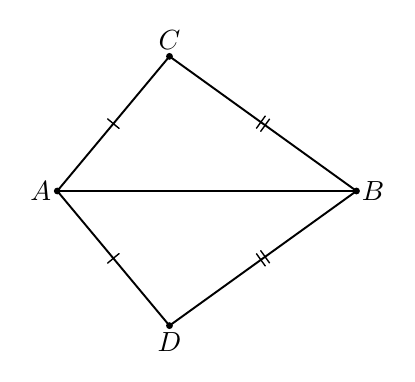
\begin{tikzpicture}[scale=0.95,line cap=round,line join=round]
  \draw[line width=0.7pt] (0.000,0.000) -- (4.000,0.000);
  \draw[line width=0.7pt] (0.000,0.000) -- (1.500,1.800);
  \draw[line width=0.7pt] (1.500,1.800) -- (4.000,0.000);
  \draw[line width=0.7pt] (0.000,0.000) -- (1.500,-1.800);
  \draw[line width=0.7pt] (1.500,-1.800) -- (4.000,0.000);
  \draw[line width=0.5pt] (0.827,0.836) -- (0.673,0.964);
  \draw[line width=0.5pt] (0.673,-0.964) -- (0.827,-0.836);
  \draw[line width=0.5pt] (2.663,0.839) -- (2.780,1.002);
  \draw[line width=0.5pt] (2.720,0.798) -- (2.837,0.961);
  \draw[line width=0.5pt] (2.780,-1.002) -- (2.663,-0.839);
  \draw[line width=0.5pt] (2.837,-0.961) -- (2.720,-0.798);
  \fill (0.000,0.000) circle (1.3pt);
  \node[anchor=center,inner sep=1pt] at (-0.220,0.000) {$A$};
  \fill (4.000,0.000) circle (1.3pt);
  \node[anchor=center,inner sep=1pt] at (4.220,0.000) {$B$};
  \fill (1.500,1.800) circle (1.3pt);
  \node[anchor=center,inner sep=1pt] at (1.500,2.020) {$C$};
  \fill (1.500,-1.800) circle (1.3pt);
  \node[anchor=center,inner sep=1pt] at (1.500,-2.020) {$D$};
\end{tikzpicture}
\end{center}

\newpage
% ===================== ĐỀ SỐ 4 =====================
\noindent
\begin{minipage}[t]{0.38\linewidth}\centering
TRƯỜNG THCS \dotfill\\[2pt]
\textbf{ĐỀ SỐ 4}
\end{minipage}\hfill
\begin{minipage}[t]{0.6\linewidth}\centering
\textbf{ĐỀ KIỂM TRA GIỮA HỌC KÌ I}\\
\textbf{NĂM HỌC 2026 -- 2027}\\
\textbf{MÔN: TOÁN 7} -- Sách \textit{Kết nối tri thức với cuộc sống}\\
\textit{Thời gian làm bài: 90 phút (không kể thời gian giao đề)}
\end{minipage}

\medskip
Họ và tên: \dotfill\ Lớp: \makebox[2cm]{\dotfill}\ Số báo danh: \makebox[2.5cm]{\dotfill}
\phan{A. TRẮC NGHIỆM (3,0 điểm)}
\textbf{Phần I. Câu trắc nghiệm nhiều phương án lựa chọn} \textit{(1,0 điểm)}. Thí sinh trả lời từ câu 1 đến câu 4. Mỗi câu hỏi thí sinh chỉ chọn một phương án.
\cau{1} Cách viết nào sau đây là đúng?
\bonpa{$-\dfrac{2}{3}\in\mathbb{N}$}{$-5\notin\mathbb{Q}$}{$\dfrac{1}{2}\in\mathbb{Z}$}{$-0{,}4\in\mathbb{Q}$}
\cau{2} Kết quả của phép tính $\left(3^{2}\right)^{4}$ là
\bonpa{$3^{6}$}{$3^{8}$}{$3^{16}$}{$9^{8}$}
\cau{3} Phân số nào sau đây viết được dưới dạng số thập phân hữu hạn?
\bonpa{$\dfrac{1}{6}$}{$\dfrac{2}{15}$}{$\dfrac{7}{40}$}{$\dfrac{5}{9}$}
\cau{4} Qua một điểm nằm ngoài một đường thẳng, có bao nhiêu đường thẳng song song với đường thẳng đó?
\bonpa{Không có.}{Chỉ có một.}{Có hai.}{Có vô số.}

\medskip\textbf{Phần II. Câu trắc nghiệm đúng sai} \textit{(1,0 điểm)}. Trong mỗi ý a), b), c), d) ở câu 5, thí sinh chọn đúng hoặc sai.
\cau{5} Cho tam giác $ABC$ có $\widehat{A}=60^\circ$ và $\widehat{B}=2\widehat{C}$.
\y{a) $\widehat{B}=60^\circ$.}
\y{b) $\widehat{B}+\widehat{C}=120^\circ$.}
\y{c) Tam giác $ABC$ là tam giác tù.}
\y{d) $\widehat{C}=40^\circ$.}

\medskip\textbf{Phần III. Câu trắc nghiệm trả lời ngắn} \textit{(1,0 điểm)}. Thí sinh trả lời từ câu 6 đến câu 9.
\cau{6} Tính $1{,}5+\left(-\dfrac{3}{4}\right)$ (viết kết quả dưới dạng số thập phân).
\cau{7} Tìm $x$, biết $2x+\dfrac{1}{2}=\dfrac{9}{2}$.
\cau{8} Tính giá trị của biểu thức $\dfrac{4^{5}}{2^{8}}$.
\cau{9} Cho $\widehat{xOy}$ và $\widehat{yOx'}$ là hai góc kề bù, $\widehat{xOy}=110^\circ$. Tia $Ot$ là tia phân giác của $\widehat{yOx'}$. Tính số đo $\widehat{tOx'}$ (đơn vị: độ).
\phan{B. TỰ LUẬN (7,0 điểm)}
\bai{1}{1,0 điểm} Tính (hợp lí nếu có thể):
\y{a) $25\cdot\left(-\dfrac{1}{5}\right)^{3}+\dfrac{1}{5}-2\cdot\left(-\dfrac{1}{2}\right)^{2}$;}
\y{b) $\dfrac{3}{5}:\left(-\dfrac{1}{15}-\dfrac{1}{6}\right)+\dfrac{3}{5}:\left(-\dfrac{1}{3}-\dfrac{16}{15}\right)$.}
\bai{2}{1,5 điểm} Tìm $x$, biết:
\y{a) $-\dfrac{5}{6}+x=\dfrac{1}{4}$;}
\y{b) $\left(x+\dfrac{1}{5}\right):\dfrac{3}{4}=-\dfrac{2}{3}$;}
\y{c) $3^{x-1}+5\cdot 3^{x-1}=162$.}
\bai{3}{1,0 điểm} Một chiếc áo có giá niêm yết là $250\,000$ đồng. Nhân dịp khai trương, cửa hàng giảm giá $\dfrac{1}{5}$ giá niêm yết. Riêng khách hàng có thẻ thành viên được giảm thêm $\dfrac{1}{10}$ giá đã giảm. Bạn An có thẻ thành viên, hỏi bạn An phải trả bao nhiêu tiền để mua chiếc áo đó?
\bai{4}{1,5 điểm} Cho hình vẽ bên, tam giác $ABC$ có $\widehat{B}=60^\circ$, $\widehat{C}=45^\circ$; đường thẳng $a$ đi qua $A$ và song song với $BC$.
\begin{center}
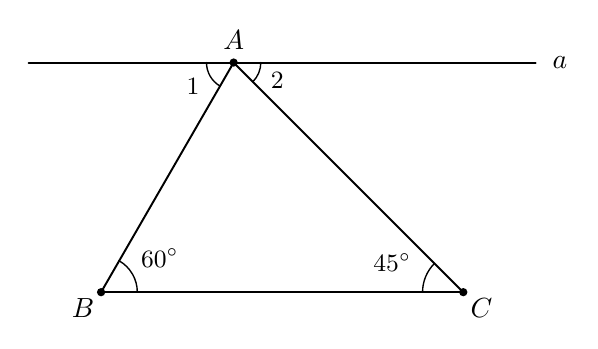
\begin{tikzpicture}[scale=1.15,line cap=round,line join=round]
  \draw[line width=0.7pt] (1.464,2.536) -- (0.000,0.000);
  \draw[line width=0.7pt] (0.000,0.000) -- (4.000,0.000);
  \draw[line width=0.7pt] (4.000,0.000) -- (1.464,2.536);
  \draw[line width=0.7pt] (-0.800,2.536) -- (4.800,2.536);
  \node[anchor=west,inner sep=1pt] at (4.950,2.536) {$a$};
  \fill (1.464,2.536) circle (1.3pt);
  \node[anchor=center,inner sep=1pt] at (1.464,2.786) {$A$};
  \fill (0.000,0.000) circle (1.3pt);
  \node[anchor=center,inner sep=1pt] at (-0.200,-0.180) {$B$};
  \fill (4.000,0.000) circle (1.3pt);
  \node[anchor=center,inner sep=1pt] at (4.200,-0.180) {$C$};
  \draw[line width=0.5pt] (0.400,0.000) arc[start angle=0,end angle=60,radius=0.400];
  \node[anchor=center,inner sep=1pt] at (0.650,0.375) {{\small $60^\circ$}};
  \draw[line width=0.5pt] (3.682,0.318) arc[start angle=135,end angle=180,radius=0.450];
  \node[anchor=center,inner sep=1pt] at (3.215,0.325) {{\small $45^\circ$}};
  \draw[line width=0.5pt] (1.164,2.536) arc[start angle=180,end angle=240,radius=0.300];
  \node[anchor=center,inner sep=1pt] at (1.014,2.276) {{\small 1}};
  \draw[line width=0.5pt] (1.676,2.324) arc[start angle=315,end angle=360,radius=0.300];
  \node[anchor=center,inner sep=1pt] at (1.945,2.337) {{\small 2}};
\end{tikzpicture}
\end{center}
\y{a) Tính số đo $\widehat{A_1}$.}
\y{b) Tính số đo $\widehat{A_2}$.}
\y{c) Tính số đo $\widehat{BAC}$.}
\bai{5}{1,5 điểm} Cho tứ giác $ABCD$ có $AB=CD$ và $AD=BC$ (như hình vẽ dưới đây).
\begin{center}
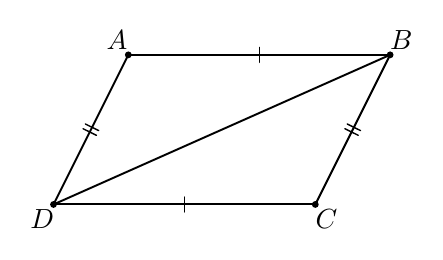
\begin{tikzpicture}[scale=0.95,line cap=round,line join=round]
  \draw[line width=0.7pt] (1.000,2.000) -- (4.500,2.000);
  \draw[line width=0.7pt] (4.500,2.000) -- (3.500,0.000);
  \draw[line width=0.7pt] (3.500,0.000) -- (0.000,0.000);
  \draw[line width=0.7pt] (0.000,0.000) -- (1.000,2.000);
  \draw[line width=0.7pt] (4.500,2.000) -- (0.000,0.000);
  \draw[line width=0.5pt] (2.750,1.900) -- (2.750,2.100);
  \draw[line width=0.5pt] (1.750,-0.100) -- (1.750,0.100);
  \draw[line width=0.5pt] (0.426,1.076) -- (0.605,0.987);
  \draw[line width=0.5pt] (0.395,1.013) -- (0.574,0.924);
  \draw[line width=0.5pt] (3.926,1.076) -- (4.105,0.987);
  \draw[line width=0.5pt] (3.895,1.013) -- (4.074,0.924);
  \fill (1.000,2.000) circle (1.3pt);
  \node[anchor=center,inner sep=1pt] at (0.850,2.200) {$A$};
  \fill (4.500,2.000) circle (1.3pt);
  \node[anchor=center,inner sep=1pt] at (4.650,2.200) {$B$};
  \fill (3.500,0.000) circle (1.3pt);
  \node[anchor=center,inner sep=1pt] at (3.650,-0.200) {$C$};
  \fill (0.000,0.000) circle (1.3pt);
  \node[anchor=center,inner sep=1pt] at (-0.150,-0.200) {$D$};
\end{tikzpicture}
\end{center}
\y{a) Chứng minh $\triangle ABD=\triangle CDB$.}
\y{b) Chứng minh $AB\parallel CD$.}
\y{c) Chứng minh $AD\parallel BC$.}
\bai{6}{0,5 điểm} Tính tổng $B=1+\dfrac{1}{2}+\dfrac{1}{2^{2}}+\dfrac{1}{2^{3}}+\ldots+\dfrac{1}{2^{100}}$.

\bigskip\begin{center}\textbf{--------- HẾT ---------}\\
\textit{Giáo viên coi kiểm tra không giải thích gì thêm.}\end{center}

\newpage
\begin{center}{\large\textbf{HƯỚNG DẪN CHẤM -- ĐỀ SỐ 4}}\end{center}
\phan{A. TRẮC NGHIỆM (3,0 điểm)}
\textbf{Phần I.} Mỗi câu trả lời đúng được 0,25 điểm.

\begin{tabular}{|l|*{4}{>{\centering\arraybackslash}p{2cm}|}}\hline
Câu & 1 & 2 & 3 & 4 \\ \hline
Đáp án & \textbf{D} & \textbf{B} & \textbf{C} & \textbf{B} \\ \hline
\end{tabular}

\textbf{Phần II.} Mỗi ý trả lời đúng được 0,25 điểm.

\begin{tabular}{|l|*{4}{>{\centering\arraybackslash}p{2cm}|}}\hline
Câu 5 & a) & b) & c) & d) \\ \hline
Đáp án & \textbf{Sai} & \textbf{Đúng} & \textbf{Sai} & \textbf{Đúng} \\ \hline
\end{tabular}

\textbf{Phần III.} Mỗi câu trả lời đúng được 0,25 điểm.

\begin{tabular}{|l|*{4}{>{\centering\arraybackslash}p{2cm}|}}\hline
Câu & 6 & 7 & 8 & 9 \\ \hline
Đáp án & \textbf{0,75} & \textbf{2} & \textbf{4} & \textbf{35} \\ \hline
\end{tabular}

\phan{B. TỰ LUẬN (7,0 điểm)}
\begin{longtable}{|>{\bfseries}c|p{0.76\linewidth}|>{\centering\arraybackslash}p{1.3cm}|}\hline
Bài & \multicolumn{1}{c|}{\textbf{Nội dung}} & \textbf{Điểm} \\ \hline\endhead
1a & \rule{0pt}{4ex}$=25\cdot\left(-\dfrac{1}{125}\right)+\dfrac{1}{5}-2\cdot\dfrac{1}{4}=-\dfrac{1}{5}+\dfrac{1}{5}-\dfrac{1}{2}$\rule[-2.4ex]{0pt}{0pt} & 0,25 \\ \hline
 & \rule{0pt}{4ex}$=-\dfrac{1}{2}$\rule[-2.4ex]{0pt}{0pt} & 0,25 \\ \hline
1b & \rule{0pt}{4ex}$=\dfrac{3}{5}:\left(-\dfrac{7}{30}\right)+\dfrac{3}{5}:\left(-\dfrac{7}{5}\right)=-\dfrac{18}{7}+\left(-\dfrac{3}{7}\right)$\rule[-2.4ex]{0pt}{0pt} & 0,25 \\ \hline
 & \rule{0pt}{4ex}$=-\dfrac{21}{7}=-3$\rule[-2.4ex]{0pt}{0pt} & 0,25 \\ \hline
2a & \rule{0pt}{4ex}$x=\dfrac{1}{4}+\dfrac{5}{6}=\dfrac{3}{12}+\dfrac{10}{12}$\rule[-2.4ex]{0pt}{0pt} & 0,25 \\ \hline
 & \rule{0pt}{4ex}$x=\dfrac{13}{12}$. Vậy $x=\dfrac{13}{12}$.\rule[-2.4ex]{0pt}{0pt} & 0,25 \\ \hline
2b & \rule{0pt}{4ex}$x+\dfrac{1}{5}=-\dfrac{2}{3}\cdot\dfrac{3}{4}=-\dfrac{1}{2}$\rule[-2.4ex]{0pt}{0pt} & 0,25 \\ \hline
 & \rule{0pt}{4ex}$x=-\dfrac{1}{2}-\dfrac{1}{5}=-\dfrac{7}{10}$. Vậy $x=-\dfrac{7}{10}$.\rule[-2.4ex]{0pt}{0pt} & 0,25 \\ \hline
2c & $3^{x-1}\cdot(1+5)=162$, suy ra $3^{x-1}=27=3^{3}$ & 0,25 \\ \hline
 & $x-1=3$, $x=4$. Vậy $x=4$. & 0,25 \\ \hline
3 & \rule{0pt}{4ex}Số tiền được giảm lần thứ nhất: $250\,000\cdot\dfrac{1}{5}=50\,000$ (đồng).\rule[-2.4ex]{0pt}{0pt} & 0,25 \\ \hline
 & Giá chiếc áo sau khi giảm lần thứ nhất: $250\,000-50\,000=200\,000$ (đồng). & 0,25 \\ \hline
 & \rule{0pt}{4ex}Số tiền bạn An được giảm thêm: $200\,000\cdot\dfrac{1}{10}=20\,000$ (đồng).\rule[-2.4ex]{0pt}{0pt} & 0,25 \\ \hline
 & Số tiền bạn An phải trả: $200\,000-20\,000=180\,000$ (đồng). & 0,25 \\ \hline
4a & Vì $a\parallel BC$ nên $\widehat{A_1}=\widehat{B}$ (hai góc so le trong) & 0,25 \\ \hline
 & Do đó $\widehat{A_1}=60^\circ$. & 0,25 \\ \hline
4b & Vì $a\parallel BC$ nên $\widehat{A_2}=\widehat{C}$ (hai góc so le trong) & 0,25 \\ \hline
 & Do đó $\widehat{A_2}=45^\circ$. & 0,25 \\ \hline
4c & Ta có $\widehat{A_1}+\widehat{BAC}+\widehat{A_2}=180^\circ$ & 0,25 \\ \hline
 & nên $\widehat{BAC}=180^\circ-60^\circ-45^\circ=75^\circ$. & 0,25 \\ \hline
5 & Ghi GT – KL đúng. & 0,25 \\ \hline
5a & Xét $\triangle ABD$ và $\triangle CDB$ có: $AB=CD$ (gt); $AD=CB$ (gt); $BD$ là cạnh chung. & 0,25 \\ \hline
 & Do đó $\triangle ABD=\triangle CDB$ (c.c.c). & 0,25 \\ \hline
5b & Từ câu a suy ra $\widehat{ABD}=\widehat{CDB}$ (hai góc tương ứng). & 0,25 \\ \hline
 & Mà $\widehat{ABD}$ và $\widehat{CDB}$ ở vị trí so le trong nên $AB\parallel CD$. & 0,25 \\ \hline
5c & Từ câu a suy ra $\widehat{ADB}=\widehat{CBD}$ (hai góc tương ứng), mà hai góc này ở vị trí so le trong nên $AD\parallel BC$. & 0,25 \\ \hline
6 & \rule{0pt}{4ex}$2B=2+1+\dfrac{1}{2}+\ldots+\dfrac{1}{2^{99}}$\rule[-2.4ex]{0pt}{0pt} & 0,25 \\ \hline
 & \rule{0pt}{4ex}$2B-B=2-\dfrac{1}{2^{100}}$. Vậy $B=2-\dfrac{1}{2^{100}}$.\rule[-2.4ex]{0pt}{0pt} & 0,25 \\ \hline
\end{longtable}
\textit{Lưu ý: Học sinh làm cách khác đúng vẫn cho điểm tối đa theo thang điểm tương ứng. Bài hình không vẽ hình hoặc vẽ hình sai không chấm phần tương ứng.}

\newpage
% ===================== ĐỀ SỐ 5 =====================
\noindent
\begin{minipage}[t]{0.38\linewidth}\centering
TRƯỜNG THCS \dotfill\\[2pt]
\textbf{ĐỀ SỐ 5}
\end{minipage}\hfill
\begin{minipage}[t]{0.6\linewidth}\centering
\textbf{ĐỀ KIỂM TRA GIỮA HỌC KÌ I}\\
\textbf{NĂM HỌC 2026 -- 2027}\\
\textbf{MÔN: TOÁN 7} -- Sách \textit{Kết nối tri thức với cuộc sống}\\
\textit{Thời gian làm bài: 90 phút (không kể thời gian giao đề)}
\end{minipage}

\medskip
Họ và tên: \dotfill\ Lớp: \makebox[2cm]{\dotfill}\ Số báo danh: \makebox[2.5cm]{\dotfill}
\phan{A. TRẮC NGHIỆM (3,0 điểm)}
\textbf{Phần I. Câu trắc nghiệm nhiều phương án lựa chọn} \textit{(1,0 điểm)}. Thí sinh trả lời từ câu 1 đến câu 4. Mỗi câu hỏi thí sinh chỉ chọn một phương án.
\cau{1} Số hữu tỉ lớn nhất trong các số sau là
\bonpa{$-0{,}6$}{$\dfrac{3}{10}$}{$-\dfrac{1}{2}$}{$\dfrac{2}{5}$}
\cau{2} Kết quả của phép tính $(-0{,}5)^{2}$ là
\bonpa{$0{,}25$}{$-0{,}25$}{$1$}{$-1$}
\cau{3} Phân số $\dfrac{5}{11}$ được viết dưới dạng số thập phân là
\bonpa{$0{,}45$}{$0{,}(45)$}{$0{,}4(5)$}{$0{,}(4)$}
\cau{4} Phần giả thiết của định lí “Nếu một đường thẳng cắt hai đường thẳng song song thì hai góc đồng vị bằng nhau” là
\motpa{Hai góc đồng vị bằng nhau.}{Hai đường thẳng song song.}{Một đường thẳng cắt hai đường thẳng song song.}{Một đường thẳng cắt hai đường thẳng.}

\medskip\textbf{Phần II. Câu trắc nghiệm đúng sai} \textit{(1,0 điểm)}. Trong mỗi ý a), b), c), d) ở câu 5, thí sinh chọn đúng hoặc sai.
\cau{5} Xét tính đúng, sai của các khẳng định sau:
\y{a) $\dfrac{7}{8}=0{,}875$.}
\y{b) Làm tròn số $12{,}467$ đến hàng phần mười ta được $12{,}4$.}
\y{c) $\dfrac{2}{3}=0{,}(6)$.}
\y{d) Phân số $\dfrac{3}{14}$ viết được dưới dạng số thập phân hữu hạn.}

\medskip\textbf{Phần III. Câu trắc nghiệm trả lời ngắn} \textit{(1,0 điểm)}. Thí sinh trả lời từ câu 6 đến câu 9.
\cau{6} Tính giá trị của biểu thức $\left(\dfrac{3}{2}\right)^{2}-\dfrac{1}{4}$.
\cau{7} Tìm $x$, biết $\dfrac{3}{5}-x=\dfrac{1}{10}$ (viết kết quả dưới dạng số thập phân).
\cau{8} Cho tam giác $ABC$ có $\widehat{A}=100^\circ$ và $\widehat{B}=\widehat{C}$. Tính số đo $\widehat{B}$ (đơn vị: độ).
\cau{9} Đường thẳng $c$ cắt hai đường thẳng song song $a$ và $b$. Biết hai góc trong cùng phía tạo thành có hiệu bằng $40^\circ$. Tính số đo góc lớn hơn (đơn vị: độ).
\phan{B. TỰ LUẬN (7,0 điểm)}
\bai{1}{1,0 điểm} Tính (hợp lí nếu có thể):
\par\noindent\begin{tabularx}{\linewidth}{@{\hspace{0.6cm}}XX@{}}a) $\dfrac{13}{17}\cdot\dfrac{-2}{5}+\dfrac{4}{17}\cdot\dfrac{-2}{5}-\dfrac{3}{5}$; & b) $\dfrac{2^{10}\cdot 3^{5}}{4^{4}\cdot 3^{4}}$.\end{tabularx}
\bai{2}{1,5 điểm} Tìm $x$, biết:
\y{a) $\dfrac{3}{4}+x=-\dfrac{1}{2}$;}
\y{b) $\left(\dfrac{2}{3}-x\right)\cdot\dfrac{5}{2}=\dfrac{5}{6}$;}
\y{c) $\left(x-\dfrac{1}{2}\right)\cdot\left(x+\dfrac{2}{3}\right)=0$.}
\bai{3}{1,0 điểm} Một bể nước dạng hình hộp chữ nhật có chiều dài $2{,}5$ m, chiều rộng $1{,}6$ m và chiều cao $1{,}2$ m. Lượng nước hiện có trong bể chiếm $\dfrac{3}{4}$ thể tích của bể. Hỏi cần bơm thêm bao nhiêu lít nước nữa để bể đầy? (Biết $1\,\mathrm{m}^{3}=1\,000$ lít.)
\bai{4}{1,5 điểm} Cho hình vẽ bên, đường thẳng $c$ cắt hai đường thẳng $a$, $b$ lần lượt tại $A$, $B$ và $\widehat{A_1}=\widehat{B_1}=110^\circ$.
\begin{center}
\begin{tikzpicture}[scale=1.15,line cap=round,line join=round]
  \draw[line width=0.7pt] (-0.300,2.000) -- (5.000,2.000);
  \draw[line width=0.7pt] (-0.300,0.000) -- (5.000,0.000);
  \draw[line width=0.7pt] (1.726,2.752) -- (3.002,-0.752);
  \node[anchor=west,inner sep=1pt] at (5.150,2.000) {$a$};
  \node[anchor=west,inner sep=1pt] at (5.150,0.000) {$b$};
  \node[anchor=west,inner sep=1pt] at (1.576,2.752) {$c$};
  \fill (2.000,2.000) circle (1.3pt);
  \node[anchor=center,inner sep=1pt] at (1.700,1.780) {$A$};
  \fill (2.728,0.000) circle (1.3pt);
  \node[anchor=center,inner sep=1pt] at (3.028,-0.220) {$B$};
  \draw[line width=0.5pt] (2.300,2.000) arc[start angle=0,end angle=110,radius=0.300];
  \node[anchor=center,inner sep=1pt] at (2.287,2.410) {{\small 1}};
  \draw[line width=0.5pt] (2.103,1.718) arc[start angle=-70,end angle=0,radius=0.300];
  \node[anchor=center,inner sep=1pt] at (2.410,1.713) {{\small 2}};
  \draw[line width=0.5pt] (3.028,0.000) arc[start angle=0,end angle=110,radius=0.300];
  \node[anchor=center,inner sep=1pt] at (3.015,0.410) {{\small 1}};
  \draw[line width=0.5pt] (2.625,0.282) arc[start angle=110,end angle=180,radius=0.300];
  \node[anchor=center,inner sep=1pt] at (2.318,0.287) {{\small 2}};
\end{tikzpicture}
\end{center}
\y{a) Chứng minh $a\parallel b$.}
\y{b) Tính số đo $\widehat{A_2}$ và $\widehat{B_2}$.}
\y{c) Tia phân giác của $\widehat{B_2}$ cắt đường thẳng $a$ tại $K$. Tính số đo $\widehat{AKB}$.}
\bai{5}{1,5 điểm} Cho hai tam giác $ABC$ và $DCB$ có $AB=DC$, $AC=DB$; hai điểm $A$ và $D$ nằm cùng phía đối với đường thẳng $BC$. Gọi $O$ là giao điểm của $AC$ và $BD$.
\y{a) Chứng minh $\triangle ABC=\triangle DCB$.}
\y{b) Chứng minh $\widehat{ABD}=\widehat{DCA}$.}
\y{c) Biết $\widehat{ACB}=40^\circ$. Tính số đo $\widehat{BOC}$ và $\widehat{AOB}$.}
\bai{6}{0,5 điểm} Tìm các số nguyên $x$ để biểu thức $A=\dfrac{2x+5}{x+1}$ có giá trị là số nguyên.

\bigskip\begin{center}\textbf{--------- HẾT ---------}\\
\textit{Giáo viên coi kiểm tra không giải thích gì thêm.}\end{center}

\newpage
\begin{center}{\large\textbf{HƯỚNG DẪN CHẤM -- ĐỀ SỐ 5}}\end{center}
\phan{A. TRẮC NGHIỆM (3,0 điểm)}
\textbf{Phần I.} Mỗi câu trả lời đúng được 0,25 điểm.

\begin{tabular}{|l|*{4}{>{\centering\arraybackslash}p{2cm}|}}\hline
Câu & 1 & 2 & 3 & 4 \\ \hline
Đáp án & \textbf{D} & \textbf{A} & \textbf{B} & \textbf{C} \\ \hline
\end{tabular}

\textbf{Phần II.} Mỗi ý trả lời đúng được 0,25 điểm.

\begin{tabular}{|l|*{4}{>{\centering\arraybackslash}p{2cm}|}}\hline
Câu 5 & a) & b) & c) & d) \\ \hline
Đáp án & \textbf{Đúng} & \textbf{Sai} & \textbf{Đúng} & \textbf{Sai} \\ \hline
\end{tabular}

\textbf{Phần III.} Mỗi câu trả lời đúng được 0,25 điểm.

\begin{tabular}{|l|*{4}{>{\centering\arraybackslash}p{2cm}|}}\hline
Câu & 6 & 7 & 8 & 9 \\ \hline
Đáp án & \textbf{2} & \textbf{0,5} & \textbf{40} & \textbf{110} \\ \hline
\end{tabular}

\phan{B. TỰ LUẬN (7,0 điểm)}
\begin{longtable}{|>{\bfseries}c|p{0.76\linewidth}|>{\centering\arraybackslash}p{1.3cm}|}\hline
Bài & \multicolumn{1}{c|}{\textbf{Nội dung}} & \textbf{Điểm} \\ \hline\endhead
1a & \rule{0pt}{4ex}$=\dfrac{-2}{5}\cdot\left(\dfrac{13}{17}+\dfrac{4}{17}\right)-\dfrac{3}{5}=\dfrac{-2}{5}\cdot 1-\dfrac{3}{5}$\rule[-2.4ex]{0pt}{0pt} & 0,25 \\ \hline
 & \rule{0pt}{4ex}$=-\dfrac{5}{5}=-1$\rule[-2.4ex]{0pt}{0pt} & 0,25 \\ \hline
1b & \rule{0pt}{4ex}$=\dfrac{2^{10}\cdot 3^{5}}{\left(2^{2}\right)^{4}\cdot 3^{4}}=\dfrac{2^{10}\cdot 3^{5}}{2^{8}\cdot 3^{4}}$\rule[-2.4ex]{0pt}{0pt} & 0,25 \\ \hline
 & $=2^{2}\cdot 3=12$ & 0,25 \\ \hline
2a & \rule{0pt}{4ex}$x=-\dfrac{1}{2}-\dfrac{3}{4}=-\dfrac{2}{4}-\dfrac{3}{4}$\rule[-2.4ex]{0pt}{0pt} & 0,25 \\ \hline
 & \rule{0pt}{4ex}$x=-\dfrac{5}{4}$. Vậy $x=-\dfrac{5}{4}$.\rule[-2.4ex]{0pt}{0pt} & 0,25 \\ \hline
2b & \rule{0pt}{4ex}$\dfrac{2}{3}-x=\dfrac{5}{6}:\dfrac{5}{2}=\dfrac{1}{3}$\rule[-2.4ex]{0pt}{0pt} & 0,25 \\ \hline
 & \rule{0pt}{4ex}$x=\dfrac{2}{3}-\dfrac{1}{3}=\dfrac{1}{3}$. Vậy $x=\dfrac{1}{3}$.\rule[-2.4ex]{0pt}{0pt} & 0,25 \\ \hline
2c & \rule{0pt}{4ex}$x-\dfrac{1}{2}=0$ hoặc $x+\dfrac{2}{3}=0$\rule[-2.4ex]{0pt}{0pt} & 0,25 \\ \hline
 & \rule{0pt}{4ex}$x=\dfrac{1}{2}$ hoặc $x=-\dfrac{2}{3}$. Vậy $x\in\left\{\dfrac{1}{2};-\dfrac{2}{3}\right\}$.\rule[-2.4ex]{0pt}{0pt} & 0,25 \\ \hline
3 & Thể tích của bể: $2{,}5\cdot 1{,}6\cdot 1{,}2=4{,}8$ ($\mathrm{m}^{3}$). & 0,25 \\ \hline
 & \rule{0pt}{4ex}Lượng nước hiện có trong bể: $4{,}8\cdot\dfrac{3}{4}=3{,}6$ ($\mathrm{m}^{3}$).\rule[-2.4ex]{0pt}{0pt} & 0,25 \\ \hline
 & Lượng nước cần bơm thêm: $4{,}8-3{,}6=1{,}2$ ($\mathrm{m}^{3}$). & 0,25 \\ \hline
 & Đổi $1{,}2\,\mathrm{m}^{3}=1\,200$ lít. Vậy cần bơm thêm $1\,200$ lít nước. & 0,25 \\ \hline
4a & Ta có $\widehat{A_1}=\widehat{B_1}=110^\circ$ & 0,25 \\ \hline
 & mà $\widehat{A_1}$ và $\widehat{B_1}$ ở vị trí đồng vị nên $a\parallel b$. & 0,25 \\ \hline
4b & $\widehat{A_2}=180^\circ-\widehat{A_1}=180^\circ-110^\circ=70^\circ$ (hai góc kề bù). & 0,25 \\ \hline
 & $\widehat{B_2}=180^\circ-\widehat{B_1}=180^\circ-110^\circ=70^\circ$ (hai góc kề bù). & 0,25 \\ \hline
4c & \rule{0pt}{4ex}Lấy điểm $E$ trên đường thẳng $b$ sao cho tia $BE$ là một cạnh của $\widehat{B_2}$. Vì $BK$ là tia phân giác của $\widehat{B_2}$ nên $\widehat{KBE}=\dfrac{70^\circ}{2}=35^\circ$.\rule[-2.4ex]{0pt}{0pt} & 0,25 \\ \hline
 & Vì $a\parallel b$ nên $\widehat{AKB}=\widehat{KBE}=35^\circ$ (hai góc so le trong). & 0,25 \\ \hline
5 & Vẽ hình, ghi GT – KL đúng. \newline \textit{(Hình vẽ ở cuối hướng dẫn chấm)} & 0,25 \\ \hline
5a & Xét $\triangle ABC$ và $\triangle DCB$ có: $AB=DC$ (gt); $AC=DB$ (gt); $BC$ là cạnh chung. & 0,25 \\ \hline
 & Do đó $\triangle ABC=\triangle DCB$ (c.c.c). & 0,25 \\ \hline
5b & Từ câu a: $\widehat{ABC}=\widehat{DCB}$ và $\widehat{ACB}=\widehat{DBC}$ (các góc tương ứng). Suy ra $\widehat{ABC}-\widehat{DBC}=\widehat{DCB}-\widehat{ACB}$, tức là $\widehat{ABD}=\widehat{DCA}$. & 0,25 \\ \hline
5c & $\widehat{OBC}=\widehat{DBC}=\widehat{ACB}=40^\circ$, $\widehat{OCB}=40^\circ$. Trong $\triangle OBC$: $\widehat{BOC}=180^\circ-40^\circ-40^\circ=100^\circ$. & 0,25 \\ \hline
 & $\widehat{AOB}=180^\circ-\widehat{BOC}=80^\circ$ (hai góc kề bù). & 0,25 \\ \hline
6 & \rule{0pt}{4ex}Điều kiện $x\neq -1$. Ta có $A=\dfrac{2(x+1)+3}{x+1}=2+\dfrac{3}{x+1}$. $A$ nguyên khi $3$ chia hết cho $x+1$.\rule[-2.4ex]{0pt}{0pt} & 0,25 \\ \hline
 & $x+1\in\{1;-1;3;-3\}$, suy ra $x\in\{0;-2;2;-4\}$ (thoả mãn). & 0,25 \\ \hline
\end{longtable}
\textit{Lưu ý: Học sinh làm cách khác đúng vẫn cho điểm tối đa theo thang điểm tương ứng. Bài hình không vẽ hình hoặc vẽ hình sai không chấm phần tương ứng.}

\textbf{Hình vẽ bài 5:}
\begin{center}
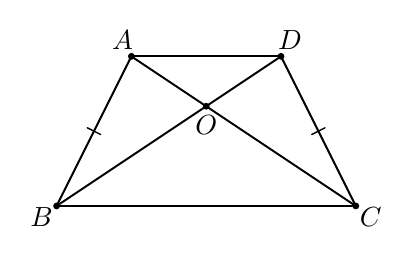
\begin{tikzpicture}[scale=0.95,line cap=round,line join=round]
  \draw[line width=0.7pt] (1.000,2.000) -- (0.000,0.000);
  \draw[line width=0.7pt] (0.000,0.000) -- (4.000,0.000);
  \draw[line width=0.7pt] (4.000,0.000) -- (3.000,2.000);
  \draw[line width=0.7pt] (1.000,2.000) -- (4.000,0.000);
  \draw[line width=0.7pt] (0.000,0.000) -- (3.000,2.000);
  \draw[line width=0.7pt] (1.000,2.000) -- (3.000,2.000);
  \draw[line width=0.5pt] (0.411,1.045) -- (0.589,0.955);
  \draw[line width=0.5pt] (3.411,0.955) -- (3.589,1.045);
  \fill (1.000,2.000) circle (1.3pt);
  \node[anchor=center,inner sep=1pt] at (0.880,2.220) {$A$};
  \fill (3.000,2.000) circle (1.3pt);
  \node[anchor=center,inner sep=1pt] at (3.120,2.220) {$D$};
  \fill (0.000,0.000) circle (1.3pt);
  \node[anchor=center,inner sep=1pt] at (-0.200,-0.150) {$B$};
  \fill (4.000,0.000) circle (1.3pt);
  \node[anchor=center,inner sep=1pt] at (4.200,-0.150) {$C$};
  \fill (2.000,1.333) circle (1.3pt);
  \node[anchor=center,inner sep=1pt] at (2.000,1.083) {$O$};
\end{tikzpicture}
\end{center}

\end{document}
